\documentclass{article}
\usepackage{pdfpages}
\usepackage{grffile}
\usepackage{graphicx}
\usepackage{fancyhdr}
\usepackage{lastpage}
\usepackage[swedish]{babel}

\pagestyle{fancy}

\lhead{Bilagor}
\rhead{Page \thepage \hspace{1pt} of \pageref{LastPage}}

\begin{document}

\title{

\includegraphics[width=0.25\textwidth]{logo.pdf} \\
Bilagor till LUDD:s medlemsmöte 2019-03-14.
}

\date{}
\author{}

\maketitle
\tableofcontents

\pagenumbering{roman}

\newcommand\blfootnote[1]{%
  \begingroup
  \renewcommand\thefootnote{}\footnote{#1}%
  \addtocounter{footnote}{-1}%
  \endgroup
}

%\blfootnote{\textbf{NOTIS: }Samtliga yrkanden är transkriberade från pappersform.}

%\includepdf[scale=0.9,pages=1,pagecommand={\section{Rapport från styrelsen},\blfootnote{\textbf{NOTIS: }Ursäkta den låga kvalitén på rapporten - John Elfberg Larsson.}}]{rapport.pdf}

\addtocounter{section}{1}
\addcontentsline{toc}{section}{\protect\numberline{\thesection}Rapport från
styrelsen}
\includepdf[scale=0.7,pages=1,pagecommand={}]{Rapport_från_styrelsen.pdf}

\addtocounter{section}{1}
\addcontentsline{toc}{section}{\protect\numberline{\thesection}Ekonomisk
redovisning}
%\includepdf[scale=0.7,pages=1,pagecommand={}]{root_motion_ap.pdf}
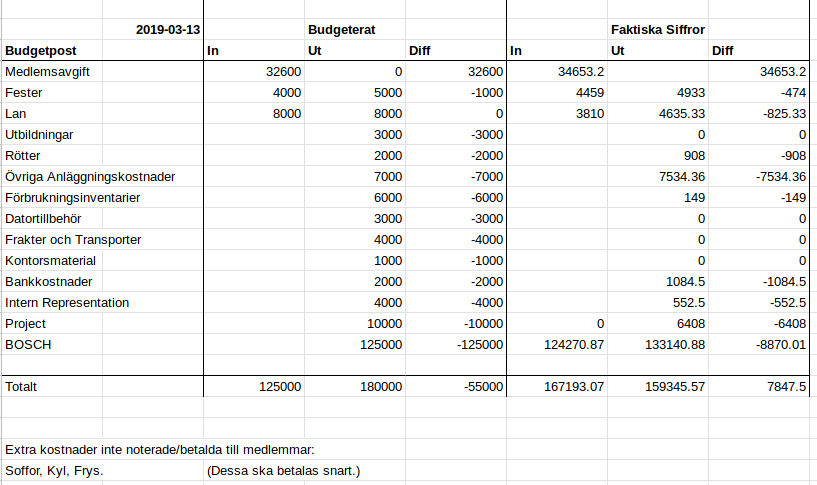
\includegraphics[scale=0.7]{money.png}
\newpage 

\addtocounter{section}{1}
\addcontentsline{toc}{section}{\protect\numberline{\thesection}Budgetförslag
verksamhetsåret 2019/2020}
%\includepdf[scale=0.7,pages=1,pagecommand={}]{root_motion_byggmaterial.pdf}
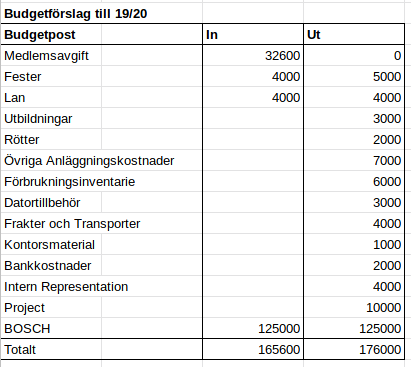
\includegraphics[scale=0.7]{money2.png}
\newpage 

\addtocounter{section}{1}
\addcontentsline{toc}{section}{\protect\numberline{\thesection}Git-diff för
uppdatering av LUDD:s mål och visioner}
%\includepdf[scale=0.7,pages=1,pagecommand={}]{root_motion_natverkskort.pdf}
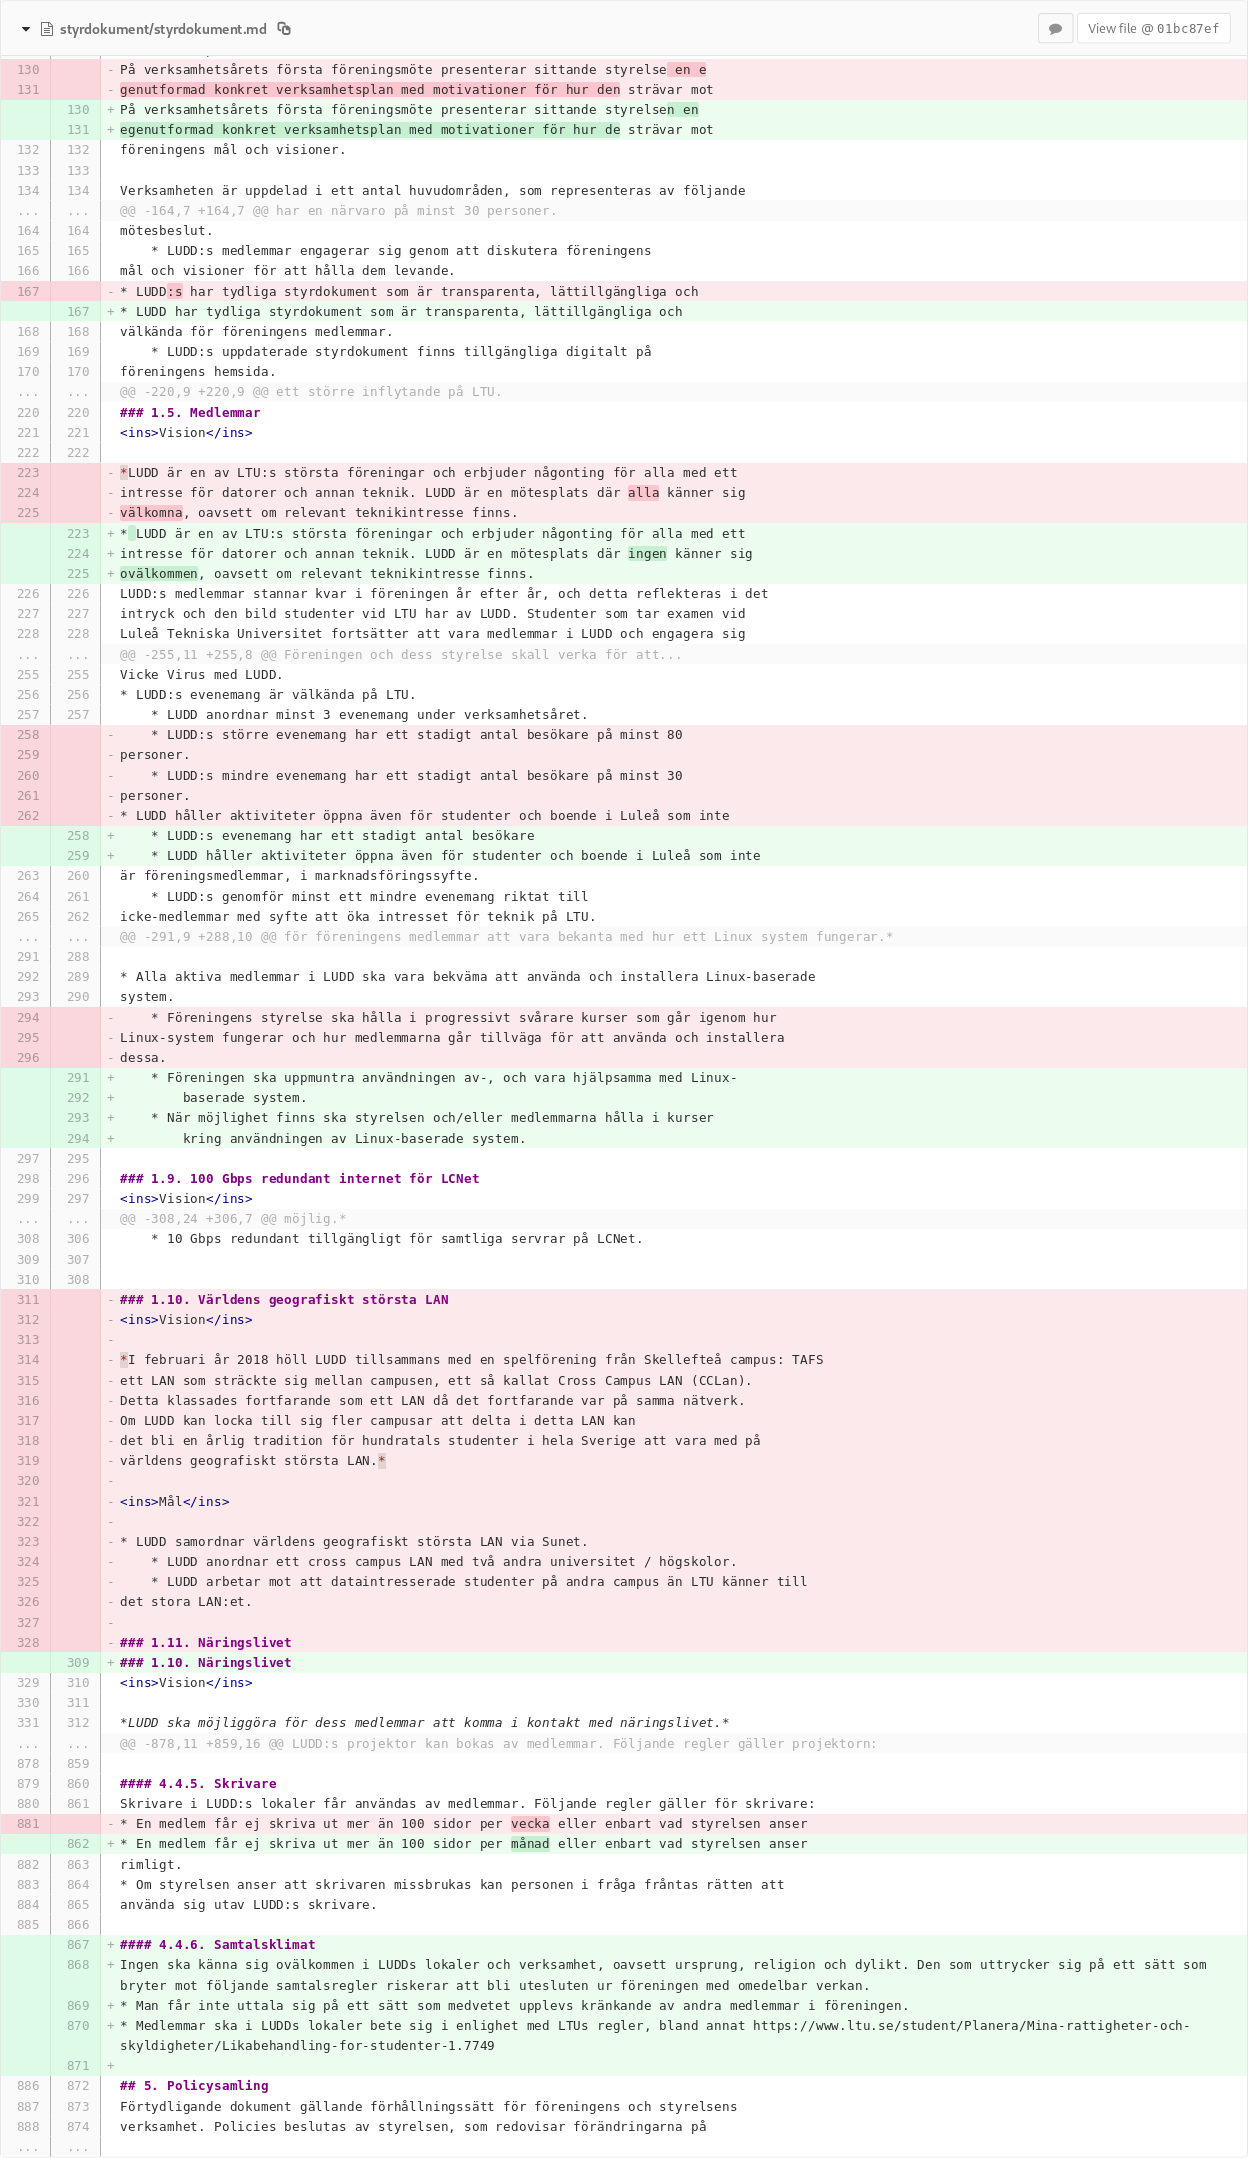
\includegraphics[]{git-diff.png}
\newpage 

\addtocounter{section}{1}
\addcontentsline{toc}{section}{\protect\numberline{\thesection}Styrelsens
tidigare beslut om tillägg av regeln "Samtalsklimat''}
%\includepdf[scale=0.7,pages=1,pagecommand={}]{root_motion_SFP.pdf}
\includegraphics[page=2, clip, trim=2.8cm 7cm 0cm 12cm, scale=0.7]{2019-02-17.pdf}

\end{document}
